%\documentclass[10pt,a4paper]{beamer}
\documentclass[xcolor=dvipsnames]{beamer} 


\usepackage[T1]{fontenc}
\usepackage[utf8]{inputenc} %caractères spéciaux
\usepackage[french]{babel} %français
\usepackage{graphicx}
\usepackage[absolute]{textpos}

\usepackage{amsmath}
\usepackage{amsfonts}
\usepackage{amssymb}

\usepackage{xspace} %symboles extensifs

%\usecolortheme[named=Seahorse]{structure} 
\usetheme{Darmstadt}
\usecolortheme{seahorse}
%\usepackage{xcolor}
%\definecolor{blue}{rgb}{0,0,1000}

\newcommand{\ket}[1]{\ensuremath{|#1\rangle}\xspace}
\newcommand{\bra}[1]{\ensuremath{\langle #1|}\xspace}
\newcommand{\an}{\hat{a}}
\newcommand{\cre}{\hat{a}^\dagger}
\newcommand{\x}{\hat{x}}
\newcommand{\p}{\hat{p}}
\newcommand{\h}{\ensuremath{\hat{H}}\xspace}
\newcommand{\blbl}{création et annihilation }
\newcommand{\ban}{\hat{b}}
\newcommand{\bcre}{\hat{b}^\dagger}
\newcommand{\fond}{\ensuremath{| \Psi_0 \rangle}\xspace}
\newcommand{\pos}[1]{\ensuremath{\mathbf{r_{#1}}}\xspace}
\newcommand{\ond}{\ensuremath{\mathbf{k}\xspace}}
\newcommand{\A}{\ensuremath{{\mathbf{A}}}\xspace}
\newcommand{\B}{\ensuremath{{\mathbf{B}}}\xspace}
\newcommand{\M}[1]{\ensuremath{\mathbf{m}(#1)}\xspace}
\newcommand{\ank}{\an_{\ond}}
\newcommand{\crek}{\cre_{\ond}}
\newcommand{\bank}{\ban_{\ond}}
\newcommand{\bcrek}{\bcre_{\ond}}
\newcommand{\gam}{\gamma(\ond{})}
\newcommand{\alcre}{\hat{\alpha}^\dagger_{\ond}}
\newcommand{\alan}{\hat{\alpha}_{\ond}}
\newcommand{\betcre}{\hat{\beta}^\dagger_{\ond}}
\newcommand{\betan}{\hat{\beta}_{\ond}}
\newcommand{\om}{\ensuremath{\Omega}\xspace}
\newcommand{\bom}{\ensuremath{\bar{\Omega}}\xspace}
\newcommand{\1}{\ensuremath{\ket{\om_1\bom_1}}\xspace}
\newcommand{\2}{\ensuremath{\ket{\om_2\bom_2}}\xspace}
\newcommand{\spinu}{\ensuremath{\ket{\uparrow}}\xspace}
\newcommand{\spind}{\ensuremath{\ket{\downarrow}}\xspace}
\newcommand{\dens}{\ensuremath{\rho_0}\xspace}
\newcommand{\dred}{\ensuremath{\rho_{red}}\xspace}
\newcommand{\tr}{\text{tr}}
\newcommand{\struc}{structure en nid d'abeilles }
\newcommand{\tilm}{\ensuremath{\tilde{M}}\xspace}

\newcommand{\can}{\hat{c}}
\newcommand{\ccre}{\hat{c}^\dagger}
\newcommand{\ene}{\hat n}
\newcommand{\imp}[1]{\ensuremath{\mathbf{p_{#1}}}\xspace}
\newcommand{\Pos}[1]{\ensuremath{\mathbf{R_{#1}}}\xspace}


\title[Entropie d'intrication dans un antiferromagnétique]{Entropie d'intrication dans un cristal antiferromagnétique bidimensionnel}
\date{Stage du 23 mai au 4 juillet 2012 au \\ \Huge{Laboratoire de Physique des Solides}}
\author{Nicolas Macé\\ \textbf{Responsable de stage :} Anuradha Jagannathan}

\begin{document}

\begin{frame}
\begin{titlepage}
\end{titlepage}
\end{frame}

%\begin{frame}
%\frametitle{Introduction : Les cristaux magnétiques}
%
%Dans de tels cristaux et à basse température, les atomes interagissent par l'intermédiaire de leur spin.
%\begin{figure}[htp]
%\centering
%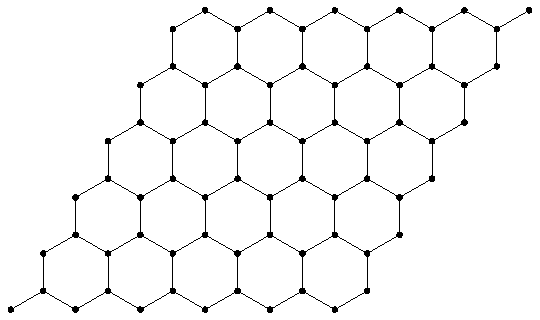
\includegraphics[scale=0.65]{vector_img/struc_nid_abeilles.pdf}
%\end{figure}
%\begin{columns}[t]
%  \begin{column}{5cm}
%  \begin{block}{}
%    \begin{figure}[htp]
%	\centering
%	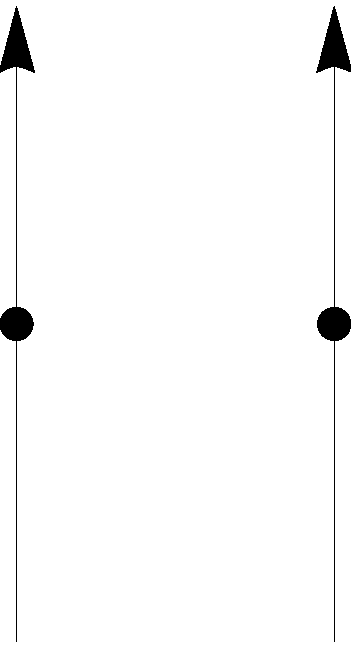
\includegraphics[scale=0.10]{vector_img/ferro.pdf}
%	\end{figure}
%	Cristal ferromagnétique.
%  \end{block} 
%  \end{column}
%  
%  \begin{column}{5cm}
%  \begin{block}{}
%	\begin{figure}[htp]
%	\centering
%	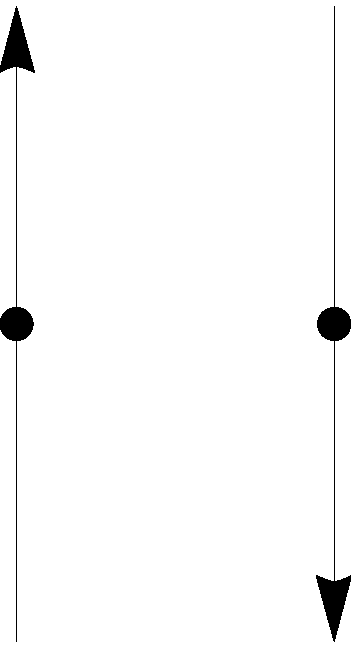
\includegraphics[scale=0.10]{vector_img/antiferro.pdf}
%	\end{figure}
%	Cristal antiferromagnétique.
%  \end{block}   
%  \end{column}
% \end{columns}
%
%\end{frame}

\begin{frame}
\frametitle{Cadre de l'étude}

\begin{columns}
\begin{column}{10cm}
\begin{block}{Hamiltonien de Heisenberg}
\centering
$\h = J\sum_{<i,j>}\mathbf{\hat S_i}\cdot\mathbf{\hat S_j}$
\end{block}
\end{column}
\end{columns}

\begin{figure}[htp]
	\centering
	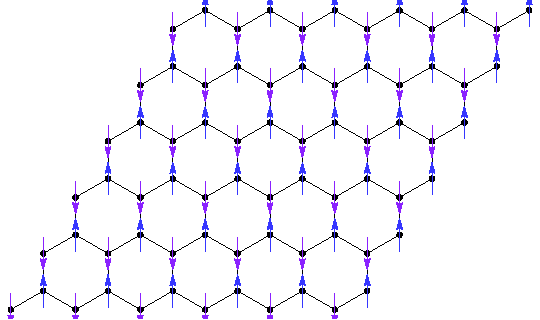
\includegraphics[scale=0.60]{vector_img/spins_struc_nid_abeilles.pdf}
\end{figure}
On étudiera un hamiltonien de Heisenberg antiferromagnétique pour une structure en nid d'abeilles bidimensionnelle.

A $T=0$ des effets d'origine quantique mal connus apparaissent. Ils se manifestent par la propriété d'\emph{intrication quantique}.
\end{frame}

\begin{frame}
\frametitle{Plan}
\tableofcontents
\end{frame}

\section{Description classique}
\begin{frame}
\frametitle{Description classique}

\begin{columns}[t]
  \begin{column}{5cm}
  \begin{center}
$\hat{\mathbf{S_i}} \rightarrow \mathbf{S_i}$
\end{center}
Spins : \emph{vecteurs} colinéaires au moment magnétique de leur atome.

\begin{center}
$\h \rightarrow E$
\end{center}

L'état fondamental classique est l'état \og spins antiparallèles \fg{}.

  \end{column}
  
  \begin{column}{5cm}
  \begin{figure}[htp]
	\centering
	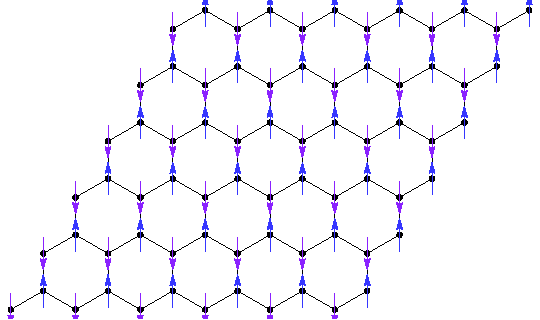
\includegraphics[scale=0.60]{vector_img/spins_struc_nid_abeilles.pdf}
	\end{figure} 
  \end{column}
 \end{columns}

\begin{columns}
\begin{column}{5cm}
\begin{alertblock}{}
L'état classique n'est pas un état propre de $\h$ !
\end{alertblock}
\end{column}
\end{columns}

\end{frame}

\section{Description quantique}
\subsection{Développement en ondes de spins}
\begin{frame}
\frametitle{Description quantique : Développement en ondes de spins}
Les spins sont maintenant des opérateurs. On veut trouver l'état fondament \fond, état propre de \h.

Ce problème n'a pas de solution analytique connue.

\begin{columns}[t]
  \begin{column}{12cm}
  \begin{block}{Transformation de Holstein-Primakoff}
    \begin{eqnarray}
    S_i^z=S-\cre_i\an_i &  
    S_i^+=\sqrt{2S}\sqrt{1-\frac{\cre_i\an_i}{2S}}\an_i &
    S_i^-=\sqrt{2S}\cre_i\sqrt{1-\frac{\cre_i\an_i}{2S}} \\
	S_i^z=-S+\bcre_i\ban_i & 
	S_i^+=\sqrt{2S}\bcre_i\sqrt{1-\frac{\bcre_i\ban_i}{2S}}\ &
	S_i^-=\sqrt{2S}\sqrt{1-\frac{\bcre_i\ban_i}{2S}}\ban_i
    \end{eqnarray}
  \end{block} 
  \end{column}
\end{columns}

\begin{columns}
  \begin{column}{12cm}
  \begin{alertblock}{Approximation $<\cre_i\an_i>\ll S$, $<\bcre_i\ban_i>\ll S$ : Développement en ondes de spins}
  	\begin{equation}
	\h_{\text{ondes de spins}}=E_{cl}+JS\sum_{<i,j>}\cre_i\an_i+\bcre_j\ban_j+\an_i\ban_j+\cre_i\bcre_j
	\end{equation}
  \end{alertblock}
  \end{column}
\end{columns}
\end{frame}

\subsection{Transformation de Bogoliubov}
\begin{frame}
\frametitle{Description quantique : transformation de Bogoliubov}

\begin{columns}
  \begin{column}{12cm}
  \begin{block}{Hamiltonien du développement en ondes de spins dans l'espace réciproque}
  	\begin{equation}
	\h=E_{cl}+JSz\sum_{\ond}\crek\ank+\bcrek\bank+\gam^*\ank\bank+\gam\crek\bcrek
	\end{equation}
  \end{block}
  \end{column}
\end{columns}

Modes propres d'excitation de cet ensemble d'oscillateurs : \emph{ondes de spins}.

Transformation de Bogoliubov : $\ank$, $\crek$ et $\bank$, $\bcrek$ $\rightarrow$ $\alan$, $\alcre$ et $\betan$, $\betcre$.
\begin{columns}
  \begin{column}{12cm}
  \begin{block}{Hamiltonien découplé après transformation de Bogoliubov}
  	\begin{equation}
	\h=E_{cl}-\frac{JSzN}{2}+JSz\sum_{\ond}E_{\ond}+JSz\sum_{\ond}E_{\ond}(\alcre\alan+\betcre\betan)
	\end{equation}
  \end{block}
  \end{column}
\end{columns}
Etat fondamental : $\alcre\alan\fond=\betcre\betan\fond=0$.
\end{frame}

\subsection{Ondes de spins et fluctuations quantiques}
\begin{frame}
\frametitle{Les ondes de spins et les fluctuations quantiques}
%\[
%	\h=E_{cl}-\frac{JSzN}{2}+JSz\sum_{\ond}E_{\ond}+JSz\sum_{\ond}E_{\ond}(\alcre\alan+\betcre\betan)
%\]
%
%\begin{itemize}
%\item $E_{\ond}=\sqrt{1-|\gam|^2}$ est l'énergie de l'onde de spin de vecteur d'onde $\mathbf{k}$.
%\item La relation de dispersion est linéaire au voisinage de $k=0$ : les ondes de spin sont alors de ondes planes qui se propagent dans tout le cristal.
%\begin{figure}[htp]
%\centering
%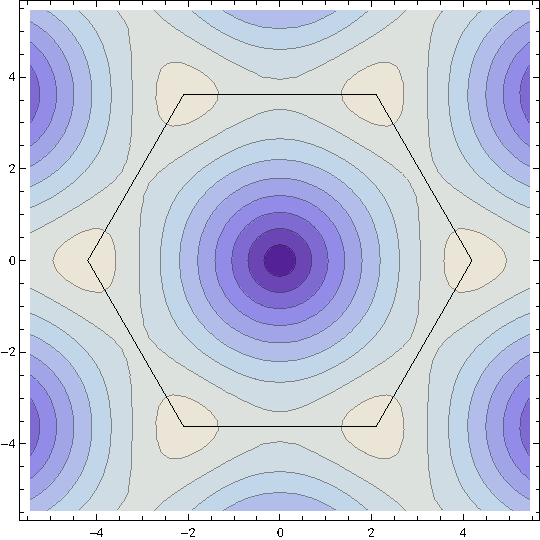
\includegraphics[scale=0.40]{vector_img/contour_energie_zone_brill.pdf}
%\end{figure}
%\end{itemize}

\[
	\h=E_{cl}-\frac{JSzN}{2}+JSz\sum_{\ond}E_{\ond}+JSz\sum_{\ond}E_{\ond}(\alcre\alan+\betcre\betan)
\]
\begin{columns}[t]
  \begin{column}{5cm}
\begin{itemize}
\item $E_{\ond}=\sqrt{1-|\gam|^2}$ est l'énergie de l'onde de spin de vecteur d'onde $\mathbf{k}$.
\item La relation de dispersion est linéaire au voisinage de $k=0$ : les ondes de spin sont alors de ondes planes qui se propagent dans tout le cristal.
\end{itemize}
  \end{column}
  
  \begin{column}{5cm}
   	\begin{figure}[htp]
	\centering
	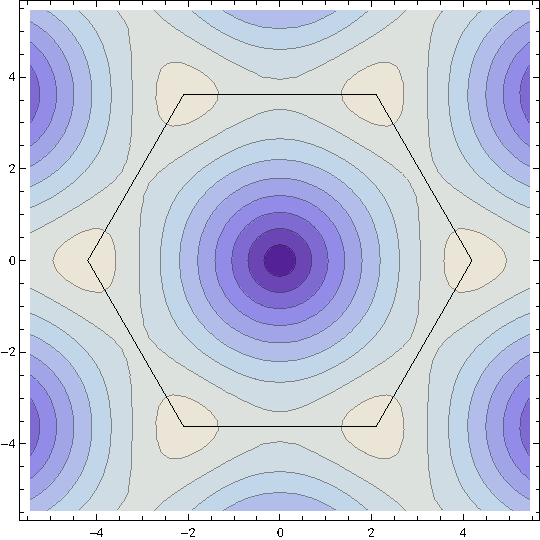
\includegraphics[scale=0.50]{vector_img/contour_energie_zone_brill.pdf}
	\end{figure}
  \end{column}
 \end{columns}
\end{frame}

\begin{frame}
\frametitle{Les ondes de spins et les fluctuations quantiques}

Énergie dans du système dans l'état fondamental : $E_{T=0}=\bra{\Psi_0}\h\fond=E_{cl}-\frac{JSzN}{2}+JSz\sum_{\ond}E_{\ond}$.


\begin{tabular}{|c|c|}
\hline
	\textbf{Type de structure} & Énergie par liaison dans l'état fondamental\\
\hline
	cristal classique & -0,25\\
\hline
	réseau carré  & -0,33\\
\hline
	structure en nid d'abeilles & -0,53\\
\hline
\end{tabular}
$\rightarrow$ fluctuations à $T=0$ autour de l'état classique \og spins antiparallèles \fg{}. Ces fluctuations sont d'origine quantique.
\end{frame}

\section{Entropie d'intrication}
%\subsection{Intrication quantique}
%\begin{frame}
%\frametitle{Intrication quantique}
%Deux spins intriqués sont décrits par une fonction d'onde collective
%\[
%\ket{\Psi}=\alpha\spinu\spind+\beta\spind\spinu
%\]
%Spin 1 mesuré $\uparrow$ : $\ket{\Psi_{spin 2}} = \spind$. Si l'on ne peut pas avoir accès à la mesure de l'état du spin 1, on a perdu de l'information.
%\begin{itemize}
%\item $\alpha=0$ ou $\beta=0$ : spins non intriqués
%\item $\alpha=\beta$ : spins \og très intriqués \fg{}
%\end{itemize} 
%L'entropie d'intrication $S$ est un nombre qui caractérise la perte d'information due à l'intrication des deux spins.
%\end{frame}

\subsection{Entropie d'intrication pour la structure antiferromagnétique en nid d'abeilles}
\begin{frame}
\frametitle{Entropie d'intrication pour la structure antiferromagnétique en nid d'abeilles}
\begin{figure}[htp]
\centering
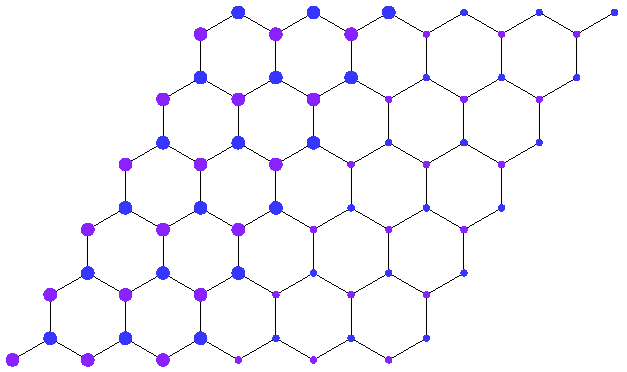
\includegraphics[scale=0.50]{vector_img/systeme_calculs.pdf}
\end{figure}
On n'a accès qu'à la partie gauche du réseau.

\begin{columns}
  \begin{column}{12cm}
  \begin{alertblock}{}
  	\begin{equation}
	S=\sum_{q} \left(\nu_q+\frac{1}{2}\right)\ln \left(\nu_q+\frac{1}{2}\right)-\left(\nu_q-\frac{1}{2}\right)\ln \left(\nu_q-\frac{1}{2}\right)
	\end{equation}
  \end{alertblock}
  \end{column}
\end{columns}
$\nu_q$ : dépend non trivialement de la géométrie du réseau.

$\rightarrow$ calculs numériques 
\end{frame}

\subsection{Résultats et interprétation}
\begin{frame}
\frametitle{Résultats et interprétation}
On a calculé l'entropie d'intrication pour des cristaux de taille $L$ croissante.
\begin{figure}[htp]
\centering
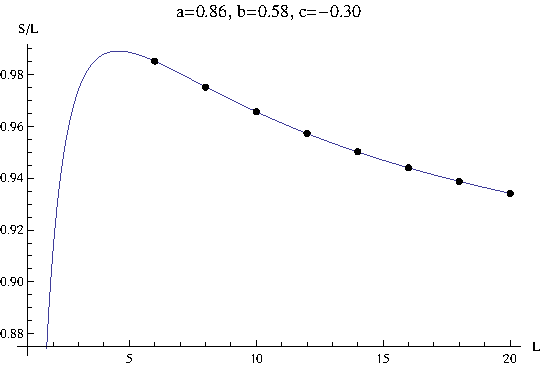
\includegraphics[scale=0.50]{vector_img/ent.pdf}
\end{figure}
Fonction d'ajustement : $S(L)=a\ln L +bL+c$

La valeur $a \simeq 0.9$ coïncide avec celle trouvée par la même méthode pour le réseau carré antiferromagnétique $ \rightarrow$ universalité ?
\end{frame}
\end{document}

